\documentclass[10pt,twocolumn,letterpaper]{article}

\usepackage{cvpr}
\usepackage{times}
\usepackage{epsfig}
\usepackage{graphicx}
\usepackage{amsmath}
\usepackage{amssymb}
% Include other packages here, before hyperref.
\usepackage[
    type={CC},
    modifier={by-nc-sa},
    version={4.0},
]{doclicense} % for licensing

\newcommand*\diff{\mathop{}\!\mathrm{d}} % helps makes typesetting calculus notation easier
\newcommand*\Diff[1]{\mathop{}\!\mathrm{d^#1}} % same as above but anything right after is a superscript

% If you comment hyperref and then uncomment it, you should delete egpaper.aux before re-running latex.  (Or just hit
% 'q' on the first latex run, let it finish, and you should be clear).
\usepackage[breaklinks=true,bookmarks=false]{hyperref}

\cvprfinalcopy % *** Uncomment this line for the final submission

\def\cvprPaperID{****} % *** Enter the CVPR Paper ID here
\def\httilde{\mbox{\tt\raisebox{-.5ex}{\symbol{126}}}}

% Pages are numbered in submission mode, and unnumbered in camera-ready \ifcvprfinal\pagestyle{empty}\fi
\setcounter{page}{1}
\begin{document}

    \title{ECE4424: Project Proposal \\ A Neural-Network Based Real-Time SISO Controller}

    \author{Mihir Savadi\\
    Bradley Department of Electrical and Computer Engineering\\
    Virginia Tech\\
    {\tt\small mihirsavadi1@vt.edu} }

    \maketitle
    \thispagestyle{empty}

    % \begin{abstract} no abstract \end{abstract}

    \section{Introduction} \label{intro}

        PID (potential, integral, derivative) control loops are ubiquitous in our world today -- it is the de-facto
        control mechanism behind ovens, toasters, home or auto HVACs, cruise controls, auto pilots, attitude control in
        drones, and various industrial processes. Its popularity is due to its simplicity, reliability, and
        interpretability -- it has been used in industry for several decades already. One drawback of the PID control
        mechanism -- and this is the focus of my project -- is that the parameters which govern them require manual
        human tuning via trial and error. In many applications this may be either extremely inconvenient, costly, or
        just infeasible. I aim to design and test an approach employing Neural-Networks (NN) that, for any system thrown
        under its purview, can automatically converge upon equivalent behavior of an ideally tuned PID control loop,
        given real-time data fed to it from the system its controlling and no human input.

        For those unfamiliar, I will first outline what PID controller's are -- they are remarkably simple. I will then
        explain my motivations for this project, after which I will detail my preliminary approach and evaluation
        metrics. Finally I will discuss the tasks and milestones I will have to achieve in order to realize my idealized
        result -- an adaptive real-time alternative to PID controllers.

    \section{PID Controllers Explained} \label{pidexplained}

        Say we had an oven that we wanted to control the temperature of. The intended temperature can be set to any
        value in a given range by a cook, and the actual temperature of the oven would then be influenced by a heating
        coil within it. This heating coil would be controlled by some electrical circuitry (often times
        mechanical!\footnote{Bimetallic strips are commonly found controlling our indicators in our cars -- making sure
        their switching frequency is constant; or the temperature control in mini-fridges.}) that would carefully
        control the power of the heating coil such that a steady temperature is maintained. If the oven is already at a
        steady temperature, and the cook increases the intended temperature, the controller would then be responsible
        for ramping up power of the coil so that the oven is able to settle at the new temperature quickly, but not
        overshoot or oscillate around it (i.e. it must ensure a \textit{perfectly damped} response). The inverse of the
        same logic applies if the cook decreased the temperature instead.

        In this example, our oven is our system that we are concerned about, which we will refer to as the
        \textbf{plant}. The output characteristic of our plant that we wish to control is the temperature, which varies
        with time -- we will refer to it as $y(t)$. The input to our plant that our controller control's in order to
        influence $y(t)$ is the power of the heating coil, which also varies with time -- we will refer to it as $u(t)$.
        The intended value of $y(t)$ -- as set by any agent, in our example the cook sets an intended temperature -- can
        also vary with time and will be referred to as $r(t)$. The error between the intended and the actual plant
        output will be referred to as $e(t)$. Eq~\ref{pideq} below defines a PID controller.
        
        \begin{equation} \label{pideq}
            \begin{gathered}
                u(t) = K_P e(t) + K_I \int_0^t e(\tau) \diff\tau + K_D \frac{\diff e(t)}{\diff t} \\
                \text{where } e(t) = r(t) - y(t)
            \end{gathered}
        \end{equation}
        
        In Section~\ref{intro} we mentioned how PID controllers have parameters that require manual tuning -- these are
        $K_P$ (called the potential), $K_I$ (called the integral), and $K_D$ (called the derivative), which can be seen
        in Eq~\ref{pideq} above. Figure~\ref{pidblock} is a block diagram representation of Eq~\ref{pideq}, which should
        help illustrate the real-time nature of this type of system. It can be observed that PID controllers are
        Single-Input Single-Output systems (SISO).
        
        \begin{figure}[h]
            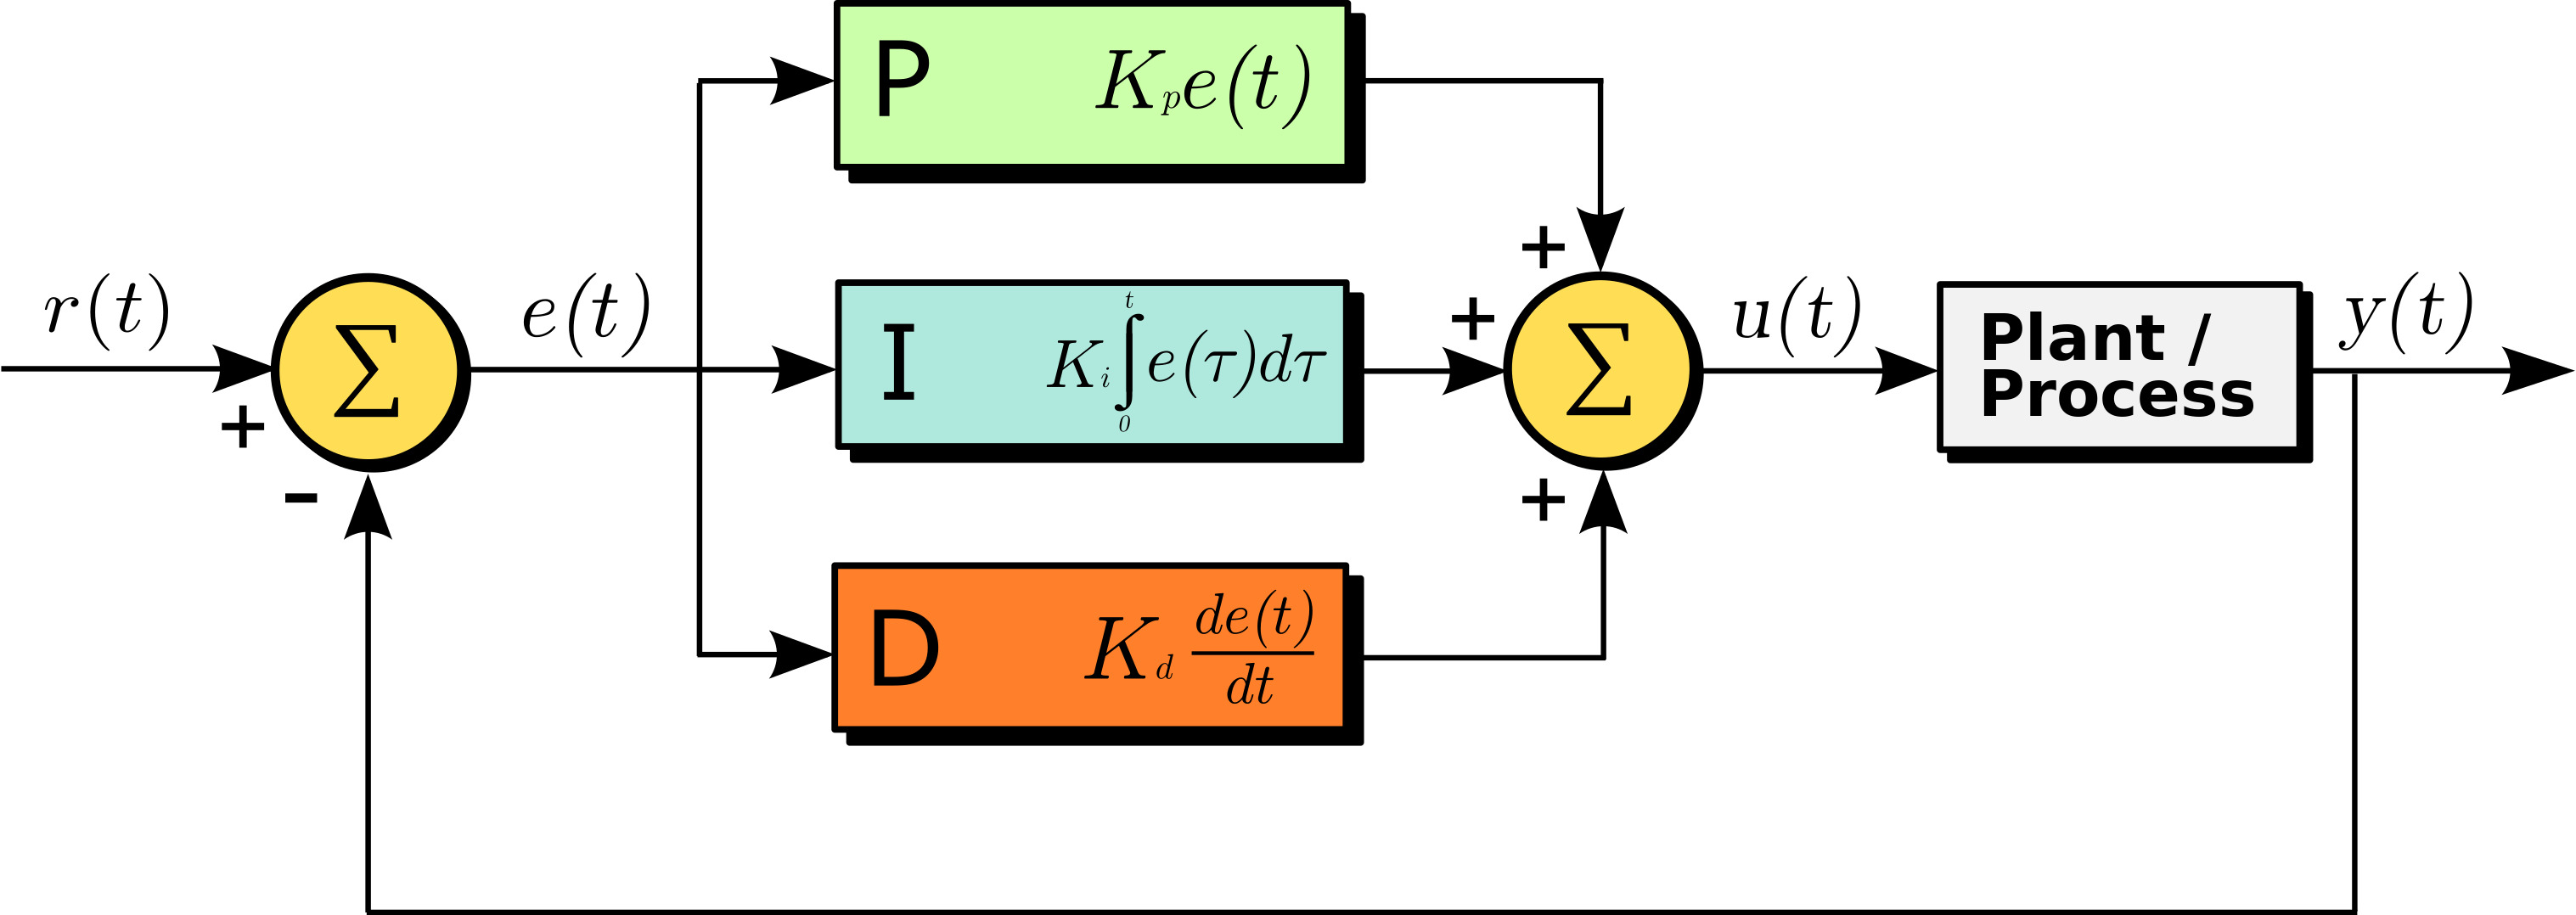
\includegraphics[width=\linewidth]{./figures/pidBlock.jpg}
            \centering
            \caption{Block diagram of a PID controller. \textit{Source:Arturo Urquizo --
            \url{https://en.wikipedia.org/wiki/PID_controller\#/media/File:PID_en.svg}}}
            \label{pidblock}
        \end{figure}

        Considering that our controller will be digital, we will be operating in discrete time. As such,
        eq~\ref{pideq_discrete} below is the `digital' version of eq~\ref{pideq}. As can be seen in
        eq~\ref{pideq_discrete}, this PID controller that we wish to emulate with our NN based approach will require
        memory (of up to $n$ samples prior to the most recent sample) of temporal information.
        
        \begin{equation} \label{pideq_discrete}
            \begin{gathered}
                u[t] = K_P e[t] + K_I \sum_{i=0}^n e[t-i] + K_D \left(e[t]-e[t-1]\right) \\
                \text{where } e[t] = r[t] - y[t], \\
                \text{and $n \geq 0$}
            \end{gathered}
        \end{equation}

    \section{Motivation} \label{motivation}
        
        In certain situations, relying on PID control systems to achieve control stability is impractical. A common
        example would be when one-off systems, that aren't massed produced and don't have R\&D time before mass
        production, need to be tuned. For example, whenever an amateur racing drone pilot builds a new custom drone with
        an off-the-shelf flight controller, they then assume the burden of tuning the PID parameters that govern their
        drone's flight characteristics. This involves flying around, observing flight behavior, and tuning iteratively
        -- this is clearly cumbersome and can even lead to situations that may damage this one-off drone. Modern flight
        control software comes with auto-tuning features, but these are mostly deterministic and perform poorly.

        Another example would be DIY reflow ovens. When hobbyists or independent printed circuit board designers want to
        build large complex boards or boards with several hard-to-hand-solder surface mount devices, they often seek the
        refuge of `reflow-ovens'. The reflow oven process involves a PCB with components placed onto their footprints
        with unsoldered `solder paste' in between. This PCB is then placed into a reflow oven, which controls the
        temperature in its chamber to follow a very specific temperature-time curve in order for the solder paste to
        melt and create sound solder joints as per the manufacturers specifications. Often times hobbyists modify
        toaster ovens into reflow ovens (which are very popular and work remarkably well) by swapping out their cheap
        mechanical controls with their own programmed PID controllers, which they then have to tune. If instead they
        could use an automatic `adaptive' controller, it would make the conversion process of any randomly chosen
        toaster oven a lot easier. 

        My personal motivation is this: I thoroughly enjoy owning and working on old cars. I recently bought a 2004 Land
        Rover Discovery II, and have since been introduced to a few people involved in the North American Land Rover
        owners communities. One of these people creates and sells kits to modernize and improve the reliability of
        certain subsystems of Discovery II's in particular. He has recently been trying to create an independent
        electrically driven air cooling system that would replace the traditional belt-driven fan systems that ship with
        not just Discovery II's, but any other car as well. This system would as a result need to monitor engine
        temperatures and adapt the power of its electrically driven fans and other cooling systems to match the thermal
        characteristics of whatever car the kit happens to be installed in, ideally without requiring the user to have
        to sit through a long and painful tuning process. From another perspective, instead of testing and shipping
        pre-tuned controllers for only a predetermined fixed set of cars -- which would require much more manual labor
        on the creators end -- an automatic `adaptive' controller would not only prevent this manual labor but also
        expand the potential market for the kit as well.

        Similar arguments from the examples above can be used to justify the benefits of such an `adaptive' controller
        in various industrial applications. As such, many efforts have been made and are currently even being
        implemented in deep industry -- please see the references section for a list of all the sources I have explored
        within this space. The approach I will be designing (detailed in Section~\ref{approach}) is not one that I have
        seen yet in existing literature, and is possibly a lot simpler than many of the approaches I have read so far.
        
    \section{Approach} \label{approach}

        The first question that arises is, on what plant\footnote{refer to Section~\ref{pidexplained} for what `plant'
        means} do I test the controller I intend to create? Initially I was going to modify a toaster oven's control
        circuitry with my own PCB involving an SSR (solid state relay), micro-controller, and other supporting
        electronics (at the time of writing this I already bought a toaster oven in anticipation, and need to return
        it). However upon further research, I found that engineers quite often emulate plants with computer models in
        order to facilitate PID and MPC (Model Predictive Controllers) control loops in software before physical
        testing. One of the models they use is called the First Order Linear System with Time Delay
        (FOPDT)\footnote{\url{https://apmonitor.com/pdc/index.php/Main/FirstOrderSystems}}
        \footnote{\url{https://apmonitor.com/pdc/index.php/Main/FirstOrderOptimization}}. Many open-source python based
        FOPDT simulators exist\footnote{\url{https://github.com/Destination2Unknown/PythonPID_Simulator}}, which I can
        easily modify to fit my own needs and controller to. This will provide a much more efficient and reliable
        platform to test my approach before diving into any hardware testing.

        The high-level structure of the NN architecture I envision is as follows. Please keep in mind that the notation
        used here will mirror what was used in Section~\ref{pidexplained}.  It will have an input layer consisting of
        multiple neurons; a single hidden layer consisting of an unknown number of neurons that I will have to
        experiment with; and an output layer consisting of a single neuron that will function as $u[t]$.

        The input layer will consist of neurons, each of which will receive inputs described in eq~\ref{inputs} as
        follows.

        \begin{equation} \label{inputs}
            \begin{gathered}
                \{r[t-k], u[t-i], y[t-i]\} \\
                \text{where } \; 0 \leq k \leq n \; \text{ and } \; 1 \leq i \leq n
            \end{gathered}
        \end{equation}

        The NN will be initialized with random weights and biases, and will undergo a specified number of rounds of back
        propagation on its entire data-set in real-time, that is at every time-step $t$. There will be no training data
        when the controller first initializes, but at every time-step $t$, a labelled data point will be appended to the
        training set -- it will have `inputs' as described in eq~\ref{inputs}, `output' $u[t]$, and error value (i.e.\
        the objective function that the gradient descent algorithm will attempt to minimize) as described in
        eq~\ref{error} below.

        \begin{equation} \label{error}
            \begin{gathered}
                e[t] = \frac{1}{z+1} \sum_{i=0}^{z} \left(r[i] - y[i]\right)^2 \\
                \text{where } \; 0 \leq z \leq n
            \end{gathered}
        \end{equation}

        The $z$ variable in eq~\ref{error} points to a time step that is somewhere in between the most recent time step
        and the beginning of time. It functions as a metric to optimize for perfect dampening of $u[t]$ to $r[t]$ within
        some specified time window $z$. If $u[t]$ is under damped, it will oscillate around $r[t]$ before converging,
        and will take a long time to converge to $r[t]$, which is what eq~\ref{error} penalizes. Similarly, if $u[t]$ is
        over damped, it will approach $r[t]$ very slowly and also take a long time to converge to $r[t]$, which
        eq~\ref{error} also penalizes. Ideally, for a given time window $z$, $e[t]$ would be as close to zero as
        possible. 
        
        Within some margin for error, $z$ needs to be adjusted to be compatible with the typical rate of change of
        $r[t]$ that the controller would experience in a particular environment. Eq~\ref{error} becomes less effective
        in quantifying quality of damping if $r[t]$ varies significantly between time-steps $t$ and $t-z$, as less time
        is given for the controller to `adapt' to changes in its input -- it is unrealistic to expect a plant to `snap'
        to an input $u[t]$; it would be impossible for an FOPDT modelled plant. Including current and previous samples
        of $r[t]$ as inputs to the NN (as described in eq~\ref{inputs}) will hopefully help with this.

        Over time, as the training set grows, the NN would adapt and `converge' towards close-to-perfectly damped
        behavior. If changes in the environment of the plant are expected, then this would be reflected by varying the
        parameters that govern the FOPDT plant simulation model in time. Training data collected before a pre-determined
        point in time can then be deleted or `forgotten', in order to allow for the NN controller to adapt.

        The ultimate goal would be to create a NN model that converges as quickly as possible to near perfect damping
        for a variety of FOPDT plant model parameter ranges. The goal would be to reduce the frequency of time-steps as
        much as possible in order to reduce the NN controller's latency which would influence its ability to `sense' the
        plant and respond quickly. Time-step frequency would be limited by how quickly the processor that the NN is
        running on can do the specified number of rounds of back propagation. A lot of variables can influence compute
        time and therefore also the time-step frequency -- the size of the training data set (which can be improved by
        controlling when old training data is `forgotten'); $k$ and $n$ from eq~\ref{inputs} and the number of neurons
        in the hidden layer directly control the number of weights and biases we have to deal with; the activation
        function we use (e.g. ReLU is much less computationally intensive than sigmoid); how large $z$ is from
        eq~\ref{error}. On the flip side, we could also argue that there could be a point of marginal returns in
        time-step frequency reduction due to NN complexity being insufficient or training data size being too small.
        Conversely, if time-step frequency is too high, $k$ and $n$ from eq~\ref{inputs} would need to be higher in
        order to capture a significantly large enough $z$ is from eq~\ref{error}, increasing compute. All these nuances
        will have to be experimented with.

        We could further speed up convergence time, instead of starting off with random weights and biases we could
        train the NN to mimic a poor performing but very general purpose PID controller. When the error value from
        eq~\ref{error} becomes small enough, we can cease training and just do inference, which would free up compute
        significantly. 

    \section{Evaluation Metrics and Milestones} \label{milestones}

        The following is a chronological list of high-level steps needed to be accomplished to achieve the desired goal
        of this project -- a functioning NN network that would converge to the performance of a manually hand tuned PID
        controller for a variety of types of FOPDT emulated plants.

        \begin{enumerate}
            \item Build FOPDT simulator code base with good abstraction so that a variety of FOPDT and controller
                varieties can be accommodated.
            \item Create a collection of FOPDT simulation scenarios and performance measurement system for automated
                controller performance testing. 
            \item Write, test, and bench mark a PID controller method in the simulator from the previous step.
            \item Write a general back propagation algorithm, or find an optimized solution off-the-shelf that is
                compatible with any arbitrary model.
            \item Write and test the novel NN controller code within the simulator from test 1. Ensure that all the
                variables discussed at the end of section~\ref{error} are easily adjustable for the sake of
                experimentation.
            \item Compile results and comparisons from steps 3 and 5 and report observations in final report.
        \end{enumerate}

    {\small
    \bibliographystyle{ieee_fullname}
    \bibliography{egbib}
    \nocite{*} % put this here to include all references without having to cite in the text
    }

    \section*{License}

        \doclicenseThis

\end{document}